% Chapter 4

\chapter{Methodology}
\label{ch:methodology}

This chapter defines the methodology used to move from a handcrafted cooperative navigation baseline to a learned trajectory predictor. The chapter is organized around four connected stages: rule-based mission execution, dataset construction, model training, and live redeployment.

\section{Methodology Overview}

The thesis follows a teacher-to-student pipeline. First, a rule-based UAV--UGV system is executed in simulation to produce stable missions, interpretable controller states, and synchronized sensing logs. Second, those runs are converted into fixed-horizon supervised trajectory samples. Third, multiple predictive models are trained on a shared split. Finally, the learned controller is reinserted into the live simulation stack and evaluated under the same mission structure as the baseline.

The design provides a classical operational reference and ensures that the learning stage is trained on data generated under the same sensing, coordination, and actuation assumptions later used at deployment time.

\section{Simulation Environment and System Setup}

All methodology stages use the Baylands simulation world, Gazebo simulation, and ROS~2 middleware. Gazebo provides robot spawning, physics, and sensor simulation. ROS~2 provides topic transport, node execution, logging, and the system interfaces needed by both the rule-based and learned pipelines. The ROS--Gazebo bridge makes the simulated signals available as standard ROS~2 topics, which allows the same execution stack to be reused during data generation and later evaluation.

The operational system contains one Husky UGV and two UAV scouts. The UGV is the only platform evaluated for mission completion. The UAVs provide persistent scout support by maintaining left and right support slots around the UGV while publishing additional context about the forward region. The same world, goal structure, topic layout, and platform set are retained when switching from the rule-based baseline to the learned-controller stage.

\section{Rule-Based Maneuver Methodology}

The rule-based baseline is a multi-node control stack rather than a single heuristic. It combines local obstacle detection, optional depth interpretation, UAV scout reporting, hazard fusion, and an explicit UGV state machine. The baseline is also the teacher that generated the later learning dataset, so the methodology must describe not only what the controller does, but also how its decisions were preserved in the recorded data.

\begin{figure}[tbp]
    \centering
    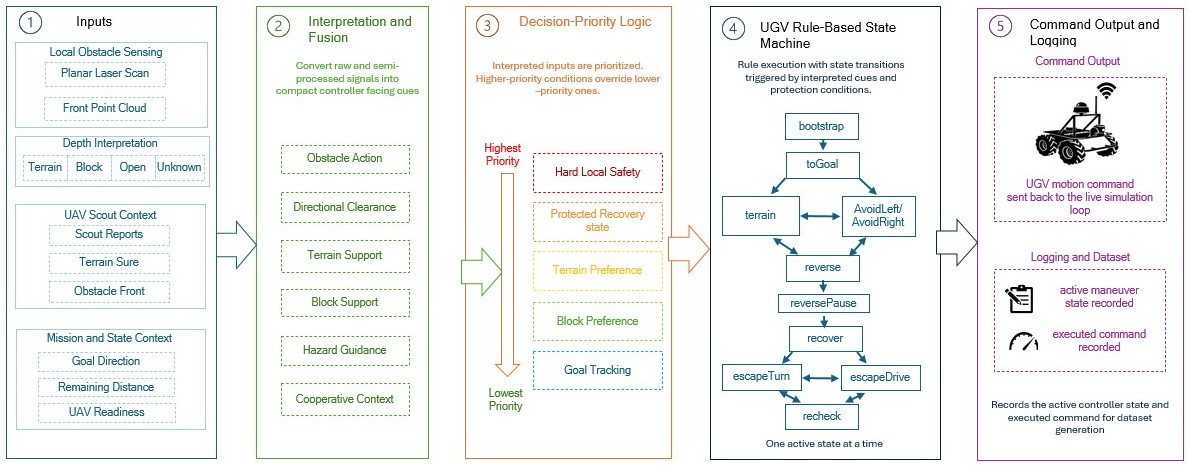
\includegraphics[width=\textwidth]{./gfx/imgae_4_1.jpg}
    \caption{Rule-based cooperative UAV--UGV maneuver methodology showing how local sensing, depth interpretation, UAV scout context, and mission-state information are transformed into compact decision cues, prioritized rule logic, state-based UGV maneuver execution, and logged teacher outputs for later dataset generation.}
    \label{fig:rule_based_maneuver_methodology}
\end{figure}

Figure~\ref{fig:rule_based_maneuver_methodology} summarizes the full rule-based maneuver pipeline. The controller first converts multi-source sensing and mission context into compact cues, applies a fixed decision-priority ordering, executes one active UGV maneuver state at a time, and records the active maneuver state and executed command for later dataset construction.

\subsection{UGV Navigation Logic}

The UGV controller executes a fixed rule sequence at each control cycle.

\begin{enumerate}
\item Validate prerequisites. If pose, goal, or required UAV readiness are unavailable, publish zero velocity.
\item Check arrival. If the remaining goal distance is below the configured tolerance of $1.5$~m, publish zero velocity and enter the \texttt{reached} state.
\item Resolve protected states first. The controller gives priority to already active recovery or transitional states such as \texttt{reverse}, \texttt{reversePause}, \texttt{recover}, \texttt{escapeTurn}, \texttt{escapeDrive}, \texttt{bootstrap}, and \texttt{terrain}.
\item Derive perception priority. The controller evaluates UAV terrain certainty, near-goal broad-block conditions, depth-image interpretation, and local obstacle status to decide whether the next decision should be terrain-biased, block-biased, or purely local.
\item Apply motion rules. If terrain is preferred, the controller enters or maintains \texttt{terrain} commitment. If obstacles dominate, it enters \texttt{avoid}. If the scene is open, it returns to direct goal tracking.
\item Apply recovery guards. Hard front blocks, zero-motion stalls, circling stalls, repeated reverse loops, and failed recovery attempts can override normal motion and force reverse, reassessment, or escape behavior.
\end{enumerate}

Table~\ref{tab:ugv_rule_summary} summarizes the main UGV rules used in the baseline runs.

\begin{table}[tbp]
    \caption{Main UGV controller states and rules used in the rule-based baseline.}
    \label{tab:ugv_rule_summary}
    \centering
    \small
    \setlength{\tabcolsep}{4pt}
    \renewcommand{\arraystretch}{1.15}
    % Column widths: c1 = 0.16\textwidth, c2 = 0.27\textwidth, c3 = remaining width (X)
    \begin{tabularx}{\textwidth}{@{}>{\raggedright\arraybackslash}p{0.16\textwidth}>{\raggedright\arraybackslash}p{0.27\textwidth}X@{}}
        \toprule
        \textbf{State / rule} & \textbf{Main trigger} & \textbf{Controller action} \\
        \midrule
        \texttt{bootstrap} & Initial $3.0$~s after start & Low-speed forward alignment, capped by a bootstrap linear speed of $0.30$~m/s. \\
        \texttt{toGoal} & No blocking condition and no active recovery & Goal-tracking command toward the shared destination. \\
        \texttt{terrain} & UAV terrain certainty, depth-supported terrain, or terrain-priority mode & Forward terrain commitment with $0.55$~m/s minimum linear speed, $\pm0.20$~rad/s angular cap, and a $2.0$~s progress timeout. \\
        \texttt{avoidLeft}/ \texttt{avoidRight} & Local obstacle action active or block-priority decision & Side-selective avoidance driven by front, left, and right clearance. \\
        \texttt{reverse} & Hard block within $0.80$~m, zero-motion stall, circling stall, or failed commit & Reverse motion for $1.5$~s. \\
        \texttt{reversePause} & End of reverse & Full stop for $2.0$~s before either recovery or escape. \\
        \texttt{recover} & Successful reverse pause exit & Short cooldown before normal goal tracking resumes. \\
        \texttt{escapeTurn} & Reverse failed to create enough displacement & In-place turn toward the wider side until approximately $\pi/2$ radians. \\
        \texttt{escapeDrive} & Escape turn completed & Straight escape drive for $3.0$~s before returning to nominal control. \\
        \texttt{recheck} & Reverse-loop guard or insufficient goal progress & Temporary pause and reassessment before re-entering \texttt{toGoal}. \\
        \bottomrule
    \end{tabularx}
\end{table}

The saved dataset preserves the controller state at the anchor frame through the \texttt{teacher\_state} field so that later samples retain the active maneuver mode at the moment the target trajectory begins.

\subsection{UAV Scout Coordination Logic}

The UAV controller is also state-based, but its role is support rather than independent mission planning. The two scouts use the same logic with mirrored lateral offsets.

\begin{enumerate}
\item \textbf{Takeoff:} each UAV climbs to the scout altitude target of $35.97$~m while loosely following the moving slot.
\item \textbf{Slot acquisition:} once near altitude, the UAV transitions to \texttt{go\_to\_slot} and converges to a slot defined by $2.5$~m forward offset and $\pm1.5$~m lateral offset relative to the Husky.
\item \textbf{Scout ready:} when the slot error falls below the $4.0$~m ready radius and the altitude error is within $1.0$~m, the UAV enters \texttt{scout\_ready} and publishes readiness plus a scout report.
\item \textbf{Obstacle and leash handling:} if a forward obstacle is detected, the UAV enters \texttt{avoid}. If it drifts beyond the Husky leash radius of $5.0$~m, it enters \texttt{return\_to\_husky} and only resumes slot tracking after the distance falls below the $4.0$~m re-entry threshold.
\item \textbf{Landing sequence:} when the Husky reaches the goal, each UAV switches to \texttt{go\_to\_land}, then \texttt{descend}, and finally \texttt{landed}.
\end{enumerate}

This design keeps the UAV contribution structured and repeatable across both rule-based execution and later dataset generation.

The nominal UAV slot is defined relative to the current Husky pose. If $\mathbf{p}_H=[x_H, y_H]^T$ and $\psi_H$ denote the Husky planar position and heading, the desired scout slot is
\[
\mathbf{p}_{\text{slot}} = \mathbf{p}_H + \mathbf{R}(\psi_H)
\begin{bmatrix}
d_f \\
\pm d_\ell
\end{bmatrix},
\qquad
\mathbf{R}(\psi_H)=
\begin{bmatrix}
\cos\psi_H & -\sin\psi_H \\
\sin\psi_H & \cos\psi_H
\end{bmatrix},
\]
where $d_f=2.5$~m is the forward offset and $d_\ell=1.5$~m is the lateral offset. The plus sign is used for one scout and the minus sign for the other, which yields the mirrored left-right support geometry around the UGV.

\subsection{Terrain and Obstacle Interpretation}

The rule-based stack interprets raw data through a sequence of compact intermediate signals. This is important because the controller does not reason directly over full lidar beams, raw point clouds, and raw depth images at every decision point. Instead, those streams are converted into smaller labels and summaries that drive the state machine.

Table~\ref{tab:data_interpretation} summarizes the main interpretation stages.

\begin{table}[tbp]
    \caption{Interpretation of raw and derived signals in the rule-based stack.}
    \label{tab:data_interpretation}
    \centering
    \small
    \setlength{\tabcolsep}{4pt}
    \renewcommand{\arraystretch}{1.15}
    % Column widths: c1 = 0.18\textwidth, c2 = 0.22\textwidth, c3 = 0.18\textwidth, c4 = remaining width (X)
    \begin{tabularx}{\textwidth}{@{}>{\raggedright\arraybackslash}p{0.18\textwidth}>{\raggedright\arraybackslash}p{0.22\textwidth}>{\raggedright\arraybackslash}p{0.18\textwidth}X@{}}
        \toprule
        \textbf{Source} & \textbf{Derived signal} & \textbf{Typical values} & \textbf{Use in the controller} \\
        \midrule
        Planar laser scan + front point cloud & Local obstacle action and directional clearance & \texttt{clear}, \texttt{turn\_left}, \texttt{turn\_right}, \texttt{caution\_left}, \texttt{caution\_right}; front/left/right distances & Immediate avoidance, caution behavior, hard-block detection, and recovery triggers. \\
        Front point cloud terrain profile & Terrain extent and climbability summary & front extent, climbable flag, effective front distance & Prevents smooth climbable terrain from being treated as a hard obstacle and enables terrain commitment. \\
        UGV depth image & Depth scene classification & \texttt{terrain}, \texttt{block\_left}, \texttt{block\_right}, \texttt{block\_center}, \texttt{block\_broad}, \texttt{open}, \texttt{unknown} & Adds a second terrain/block vote when local geometry is ambiguous. \\
        UAV scout reports & Forward scout observations & distance, lateral offset, blocked flag & Supplies aerial preview information to the hazard fusion layer. \\
        Hazard fusion & UGV-facing hazard guidance & \texttt{terrain\_sure\_front}, \texttt{obstacle\_front}, \texttt{clear} & Supports terrain override when two scouts indicate a broad, non-central front region. \\
        Optional UGV decision fuser & Final fused label & \texttt{terrain}, \texttt{block\_left}, \texttt{block\_right}, \texttt{block\_center}, \texttt{clear} & Optional controller-facing fusion of local, hazard, and depth inputs; disabled in the default dataset-generation runs. \\
        \bottomrule
    \end{tabularx}
\end{table}

The obstacle detector marks \texttt{turn\_*} when the effective front clearance falls below $1.8$~m and \texttt{caution\_*} when it falls below $3.0$~m in the live detector, while the Husky controller itself uses an obstacle caution threshold of $3.2$~m and a strict reverse threshold of $0.80$~m. The depth classifier divides the image into left, center, and right regions and applies a consensus override so that broad, smooth, front-facing terrain is not mistaken for a narrow local block. The hazard builder promotes paired left/right UAV detections into \texttt{terrain\_sure\_front} when the pattern is wide, aligned, and sufficiently far from a strong central obstruction.

\subsection{Decision Priority and Maneuver Switching}

The UGV does not assign equal authority to all signals. Its priority order is explicit:

\begin{enumerate}
\item hard local protection and active recovery states;
\item UAV-supported terrain certainty;
\item near-goal broad-block protection;
\item depth-supported block or terrain interpretation;
\item local-only obstacle handling;
\item nominal goal tracking.
\end{enumerate}

This ordering is implemented through the controller's perception-priority function. If UAV terrain certainty is active, the controller switches to terrain preference. If the UGV is near the goal and depth plus hazard cues indicate a broad block, block preference dominates. If neither special case applies, the controller falls back to depth support and then to local obstacle status.

\subsection{Recovery and Safety Logic}

Recovery is treated as a first-class part of the baseline, not as an afterthought. Four protection mechanisms are especially important:

\begin{enumerate}
\item \textbf{Strict reverse:} repeated hard front blocking forces reverse.
\item \textbf{Zero-motion reverse:} if the robot remains nearly stationary for too long, reverse is triggered even without a new obstacle event.
\item \textbf{Circling reverse:} large heading change with negligible translation is interpreted as oscillatory trapping and also triggers reverse.
\item \textbf{Loop reassessment:} repeated reverse events inside a short time window force a pause-and-reassess state.
\end{enumerate}

If reversing does not create enough displacement, the controller escalates to an escape turn followed by a short straight escape drive.

\section{Data Collection and Dataset Preparation}

The learning dataset was generated entirely from rule-based runs. No manual annotation was introduced. Each sample therefore inherits the state structure, sensor assumptions, and coordination logic of the executed baseline.

\subsection{Rule-Based Run Generation}

The saved training artifact used six recorded rule-based episodes. After frame export, those runs produced six ordered episode streams containing 44{,}625 synchronized frames in total.

\subsection{Bag Recording and Run Logging}

Each run was preserved through ROS bag recording, human-readable run logs, and episode metadata. The bag files store the machine-readable topic history. The logs preserve the operational timeline, including controller states and runtime events. The metadata makes each run self-describing for later export and comparison.

\subsection{Episode-Frame Extraction}

The bag history was exported into a restart-safe intermediate format: one \texttt{frames.jsonl} file and one manifest per episode. Each frame stores synchronized ego state, goal-relative quantities, obstacle summaries, agent context, teacher command, and teacher state. This intermediate representation decouples live simulation from later training, because sliding-window sampling and model training can be repeated without rerunning Gazebo.

\subsection{Sliding-Window Sample Generation}

Samples are produced by sliding a fixed window over each episode stream. With a past horizon of 10 frames and a future horizon of 5 frames, the number of usable windows for an episode of length $L$ is
\[
\text{usable windows} = L - 10 - 5 + 1 = L - 14.
\]
Applying this rule to the six exported episodes produced 44{,}541 supervised samples from 44{,}625 total frames.

The future target is stored in the anchor ego-local frame rather than in the world frame. If $\mathbf{p}_a=[x_a, y_a]^T$ and $\psi_a$ denote the anchor position and heading, and $\mathbf{p}^{(k)}_{\text{world}}$ is the $k$-step future world-frame UGV position, the local target is
\[
\mathbf{p}^{(k)}_{\text{local}} =
\mathbf{R}(-\psi_a)\left(\mathbf{p}^{(k)}_{\text{world}} - \mathbf{p}_a\right),
\qquad k \in \{1,\dots,5\}.
\]
This removes unnecessary global-orientation variation and keeps the supervision aligned with the local control problem.

Each sample stores only compact metadata plus the future local target. The past context is reconstructed on demand from the indexed episode stream. Table~\ref{tab:sample_record_structure} shows the structure of one saved sample record.

\begin{table}[tbp]
    \caption{Structure of one sample entry in the saved trajectory sample table.}
    \label{tab:sample_record_structure}
    \centering
    \small
    \setlength{\tabcolsep}{4pt}
    \renewcommand{\arraystretch}{1.15}
    % Column widths: c1 = 0.20\textwidth, c2 = 0.22\textwidth, c3 = remaining width (X)
    \begin{tabularx}{\textwidth}{@{}>{\raggedright\arraybackslash}p{0.20\textwidth}>{\raggedright\arraybackslash}p{0.22\textwidth}X@{}}
        \toprule
        \textbf{Field} & \textbf{Saved form} & \textbf{Meaning} \\
        \midrule
        \texttt{sample\_id} & \texttt{run\_model\_...\_start00000} & Unique sliding-window identifier. \\
        \texttt{episode\_id} & \texttt{run\_model\_20260511\_202309} & Source episode for the sample. \\
        \texttt{stream\_index} & scalar integer & Episode-stream index in the exported frame set. \\
        \texttt{start\_index} & scalar integer & First frame of the past window. \\
        \texttt{anchor\_index} & scalar integer & Final frame of the past window and reference frame for target generation. \\
        \texttt{past\_len} / \texttt{future\_len} & 10 / 5 & Fixed history and prediction horizons. \\
        \texttt{anchor\_timestamp\_ns} & 64-bit integer & Timestamp of the anchor frame. \\
        \texttt{teacher\_state} & \texttt{terrain} & Controller state at the anchor frame. \\
        \texttt{future\_xy\_local} & $5 \times 2$ float array & Future UGV displacements in the anchor ego-local $(x,y)$ frame. \\
        \texttt{future\_dt} & length-5 float array & Time offsets from the anchor frame to each predicted step. \\
        \bottomrule
    \end{tabularx}
\end{table}

Each saved sample therefore links one fixed history window to one fixed local future trajectory target.

\subsection{Shared Train, Validation, and Test Split}

All models use one fixed split produced with seed 42 and nominal ratios of 70\% training, 15\% validation, and 15\% test. The split is episode-based: the unique episode IDs are collected, shuffled with the fixed seed, assigned to partitions at episode level, and then mapped back to sample indices. Entire episodes therefore remain inside one partition, which prevents overlapping temporal windows from the same mission from appearing in both training and evaluation.

Table~\ref{tab:shared_split_summary} shows the actual split used by all notebooks.

\begin{table}[tbp]
    \caption{Shared episode-based split used by all model notebooks.}
    \label{tab:shared_split_summary}
    \centering
    \small
    \setlength{\tabcolsep}{4pt}
    \renewcommand{\arraystretch}{1.15}
    % Column widths: c1 = 0.12\textwidth, c2 = 0.13\textwidth, c3 = remaining width (X), c4 = 0.12\textwidth, c5 = 0.08\textwidth
    \begin{tabularx}{\textwidth}{@{}>{\raggedright\arraybackslash}p{0.12\textwidth}>{\raggedright\arraybackslash}p{0.13\textwidth}X>{\raggedright\arraybackslash}p{0.12\textwidth}>{\raggedright\arraybackslash}p{0.08\textwidth}@{}}
        \toprule
        \textbf{Partition} & \textbf{Episodes} & \textbf{Episode IDs} & \textbf{Samples} & \textbf{Share} \\
        \midrule
        Train & 4 & \texttt{run\_model\_20260511\_220103}, \texttt{run\_model\_20260511\_210809}, \texttt{run\_model\_20260511\_213251}, \texttt{run\_model\_20260511\_221726} & 29{,}379 & 65.96\% \\
        Validation & 1 & \texttt{run\_model\_20260511\_202309} & 6{,}195 & 13.91\% \\
        Test & 1 & \texttt{run\_model\_20260511\_222947} & 8{,}967 & 20.13\% \\
        \bottomrule
    \end{tabularx}
\end{table}

\section{Learning-Based Trajectory Prediction Methodology}

The learning stage predicts a short future UGV trajectory from recent history and compact cooperative context. The model does not learn directly from raw images or full lidar scans. Instead, it learns from structured features that mirror the signals already used by the rule-based system.

\subsection{Learning Objective}

The learning objective is short-horizon trajectory forecasting. Given recent context over the past 10 frames, the model predicts the next 5 ego-local $(x,y)$ positions of the UGV. This was preferred over direct command imitation because a short future path is smoother, easier to evaluate, and easier to convert back into live control.

\subsection{Input Representation}

The input representation contains up to four tensors, depending on the model family. The goal-and-state sequence is always present. Clearance history is added for CNN-based models. Node and edge sequences are added for graph-enabled models. Table~\ref{tab:model_input_summary} summarizes the actual tensor layout used in the implementation.

\begin{table}[tbp]
    \caption{Structured learning inputs used by the trajectory models.}
    \label{tab:model_input_summary}
    \centering
    \small
    \setlength{\tabcolsep}{4pt}
    \renewcommand{\arraystretch}{1.15}
    % Column widths: c1 = 0.17\textwidth, c2 = 0.18\textwidth, c3 = remaining width (X)
    \begin{tabularx}{\textwidth}{@{}>{\raggedright\arraybackslash}p{0.17\textwidth}>{\raggedright\arraybackslash}p{0.18\textwidth}X@{}}
        \toprule
        \textbf{Tensor} & \textbf{Shape per sample} & \textbf{Content} \\
        \midrule
        \texttt{goal\_seq} & $10 \times 13$ & Ego linear and angular motion, goal-relative position, goal distance, goal heading error, previous teacher command, and normalized front/left/right clearance. \\
        \texttt{scan\_seq} & $10 \times 3$ & Ordered front, left, and right clearance values across the past horizon. \\
        \texttt{node\_seq} & $10 \times 3 \times 12$ & Graph node features for \texttt{ego}, \texttt{uav1}, and \texttt{uav2}. \\
        \texttt{edge\_seq} & $10 \times 3 \times 3 \times 8$ & Pairwise edge features: relative displacement, distance, inverse distance, bearing sine/cosine, and self-edge indicator. \\
        \bottomrule
    \end{tabularx}
\end{table}

The goal-and-state vector has 13 features. The clearance strip has 3 features. Each graph node has 12 features, and each directed edge has 8 features. The graph node order is fixed as \texttt{ego}, \texttt{uav1}, and \texttt{uav2} at every time step.

\subsection{Output Trajectory Representation}

The output is a $5 \times 2$ local trajectory segment. Each row is the predicted future displacement of the UGV in the anchor ego-local frame. Using the local frame removes unnecessary global-orientation variation and keeps the prediction aligned with the immediate control problem faced by the live controller.

\subsection{Model Families}

Five model families were evaluated.

\begin{enumerate}
\item \textbf{Constant-velocity baseline:} deterministic extrapolation from recent local motion.
\item \textbf{CNN--LSTM:} goal/state sequence plus clearance-strip encoding.
\item \textbf{CNN--GNN--LSTM:} CNN clearance encoder, graph encoder, and recurrent temporal model.
\item \textbf{CNN--GNN--Transformer:} CNN clearance encoder, graph encoder, and transformer temporal model.
\item \textbf{CNN--GNN--LSTM--Transformer:} hybrid recurrent and transformer temporal modeling on top of the same structured inputs.
\end{enumerate}

The methodological role of each model family is defined here by its input structure and temporal formulation. A comparative interpretation of what each architectural component contributed is deferred to Chapter~6.

\section{Model Training Procedure}

The training workflow was designed to be reproducible and restart-safe. Shared artifacts are created once, stored on disk, and then reused across notebooks. Each model notebook loads the same sample table and the same fixed split before training.

\subsection{Training Configuration}

The training configuration was held constant across the main model families. Table~\ref{tab:training_config_summary} lists the actual values extracted from the notebooks.

\begin{table}[h]
    \caption{Common training configuration used in the 08 model notebooks.}
    \label{tab:training_config_summary}
    \centering
    \small
    \setlength{\tabcolsep}{4pt}
    \renewcommand{\arraystretch}{1.15}
    % Column widths: c1 = 0.42\textwidth, c2 = remaining width (X)
    \begin{tabularx}{\textwidth}{@{}>{\raggedright\arraybackslash}p{0.42\textwidth}X@{}}
        \toprule
        \textbf{Configuration item} & \textbf{Value} \\
        \midrule
        Random seed & 42 \\
        Past horizon / future horizon & 10 frames / 5 frames \\
        Target split ratios & 0.70 training / 0.15 validation / remaining test \\
        Batch size & 64 \\
        Maximum epochs & 30 \\
        Early-stopping patience & 5 epochs \\
        Learning rate & $1 \times 10^{-3}$ \\
        Weight decay & $1 \times 10^{-4}$ \\
        Hidden dimension & 128 \\
        Graph hidden dimension & 96 \\
        Dropout & 0.10 \\
        Graph message-passing steps & 2 \\
        \bottomrule
    \end{tabularx}
\end{table}

\subsection{Loss Function and Optimization}

All trainable models use the Adam optimizer and optimize a SmoothL1 trajectory loss between the predicted local path and the ground-truth local path. This choice gives stable regression behavior while remaining less sensitive to occasional larger deviations than a purely squared-error objective.

For a prediction horizon of $F=5$ future steps, the loss is computed over the local $(x,y)$ trajectory as
\[
\mathcal{L}_{\text{traj}} =
\frac{1}{2F}
\sum_{k=1}^{F}
\sum_{j \in \{x,y\}}
\operatorname{SmoothL1}\!\left(\hat{y}_{k,j} - y_{k,j}\right),
\]
where $\hat{y}_{k,j}$ and $y_{k,j}$ are the predicted and target local coordinates at future step $k$. The loss is applied directly to the future ego-local path rather than to intermediate controller states.

\subsection{Early Stopping Strategy}

Validation is performed after every epoch. The stopping criterion is validation ADE. Whenever ADE improves, the best state is saved. If ADE does not improve for five consecutive epochs, training stops early. This aligns model selection with the primary forecasting objective rather than with training loss alone.

\subsection{Checkpointing and Restart-Safe Workflow}

Each run writes a manifest, training-history CSV, plots, timestamped weights, and a \texttt{latest.pt} checkpoint. This makes the workflow restart-safe at two levels. First, shared artifacts such as episode frames, sample tables, and split files are preserved. Second, each training run preserves the exact best validation checkpoint later used for offline testing and live redeployment.

\subsection{Runtime and Resource Logging During Training}

Notebook-level runtime logging is integrated directly into the helper library. Each major stage records wall-clock start and end time, elapsed duration, system CPU, process CPU, process memory, and GPU memory statistics when CUDA is available. The runtime logger writes both a summary JSON file and a sampled CSV trace.

\section{Simulation Evaluation Method}

Evaluation is split into offline prediction testing and online live simulation.

\subsection{Offline Evaluation Procedure}

Offline evaluation loads the best validation checkpoint and applies it to the held-out test split. For each model, predicted local trajectories are compared against the saved target trajectories using ADE, FDE, and RMSE. Prediction exports and history files are written to disk for later analysis.

\subsection{Online Simulation Evaluation Procedure}

Online evaluation loads a trained checkpoint into the live controller stack. The learned controller receives the same compact live context used at training time, predicts a short future trajectory, and converts that trajectory into executable UGV motion commands. The surrounding ROS~2, UAV, and logging infrastructure remains unchanged so that the comparison with the rule-based baseline is fair.

\subsection{Rule-Based Baseline Evaluation}

The rule-based baseline is evaluated as a complete mission controller. It provides the operational reference and the teacher trajectories used to construct the learning dataset.

\subsection{Learned-Controller Evaluation}

The learned-controller stage keeps the same world, agents, and mission structure, but replaces the UGV maneuver generator with the trained predictor.

\section{Performance Metrics}

The methodology uses several metric groups because predictive quality and operational usefulness are not identical.

\subsection{Trajectory Prediction Metrics}

Offline prediction is measured with average displacement error (ADE), final displacement error (FDE), and root mean square error (RMSE). ADE measures average path agreement across the full horizon, FDE measures the final predicted point, and RMSE provides a regression-style aggregate error.

For a predicted trajectory $\hat{\mathbf{p}}_k$ and ground-truth trajectory $\mathbf{p}_k$ over $F$ future steps, the main offline metrics are
\[
\operatorname{ADE} =
\frac{1}{F}\sum_{k=1}^{F}
\left\lVert \hat{\mathbf{p}}_k - \mathbf{p}_k \right\rVert_2,
\]
\[
\operatorname{FDE} =
\left\lVert \hat{\mathbf{p}}_F - \mathbf{p}_F \right\rVert_2,
\]
\[
\operatorname{RMSE} =
\sqrt{
\frac{1}{2F}
\sum_{k=1}^{F}
\sum_{j \in \{x,y\}}
\left(\hat{y}_{k,j} - y_{k,j}\right)^2 }.
\]

\subsection{Navigation Performance Metrics}

Live evaluation additionally tracks mission-level behavior such as goal reach, remaining distance, oscillation, stability, and recovery activity. These metrics capture properties that are not visible in offline forecasting scores alone.

\subsection{Resource and Runtime Metrics}

Both training and simulation record elapsed time, CPU load, and memory footprint. GPU memory is also recorded during training when available. These measurements support the later edge-device discussion.

\subsection{Communication Metrics}

When communication-aware evaluation is enabled, the system records RSSI, SNIR, packet error rate, and link distance from the OMNeT++ bridge. These metrics are used only in the communication-aware live experiments.

\section{Resource and Runtime Measurement Method}

For simulation runs, measurement begins when the Gazebo clock starts advancing after Play and ends automatically when the UGV reaches the goal. This excludes idle session time and captures only the active mission window. CPU and memory statistics are sampled continuously and written to both summary and trace files. The same timing definition is used for the rule-based and learned-controller stacks.

For training runs, the notebook logger applies the same idea at stage level: start time, end time, elapsed time, CPU, memory, and GPU usage are recorded automatically for the major data-loading and training cells.

\section{Communication-Aware Evaluation Method}

The communication-aware extension couples the live navigation stack to an external OMNeT++ communication model. Platform poses are exported from Gazebo to the communication layer and network metrics are returned to ROS~2 through a bridge. This choice is consistent with the communication-simulation role described by \citeauthor{varga2008omnet} \citep{varga2008omnet}.

In the learned-controller stage, those communication metrics do not replace the motion policy. Instead, they modify how much trust the controller assigns to UAV-related cooperative context. Poor link quality reduces the effective weight of UAV support; better communication preserves it. This keeps the navigation architecture unchanged while making the live experiment sensitive to degraded inter-agent communication.

Overall, the methodology starts from a rule-based cooperative controller, converts its executed behavior into a structured trajectory dataset, trains multiple forecasting models under a fixed configuration, and redeploys those models into the same live simulation framework.
